\chapter{Test Results}
\label{cha:pierwszyDokument}

\section{First Set of Tests}
\label{sec:first_set_of_tests}

First set of tests uses historical data from year 2009 (data of 3 different stocks have been used). 
Portfolio contained 3 assets (they are one of the biggest companies present on WSE):

\begin{itemize} 
  \item KGHM
  \item TPSA
  \item PKO
\end{itemize}

Multi-agent platform has been used to run algorithms.
It was configured in the following way: 

\begin{itemize}
  \item configured to simulate trading strategy throughout the entire year 2009
  \item all investing decisions are solely based on results from algorithms
  \item migration mechanism between Computing Nodes has been enabled
  \item two Computing Nodes (with appropriate algorithms) have been used to obtain results
\end{itemize}

Trend following algorithm has been tested without multi-agent running platform as it is a standalone R script.

\subsection{Trend Following}

\subsubsection{Short-term trend results}

As described in \ref{trend_following_impl} and \ref{sec:trendFollowing}, we can adjust our trading rules to seek out short-term trends
 (by changing the values of $N$ and $M$ in the \emph{Simple Moving Average} method).
With values $N = 10$, $M = 20$ the SMA method focused on short-term trends.
 

\begin{figure}[ht]
  
  \begin{center}
    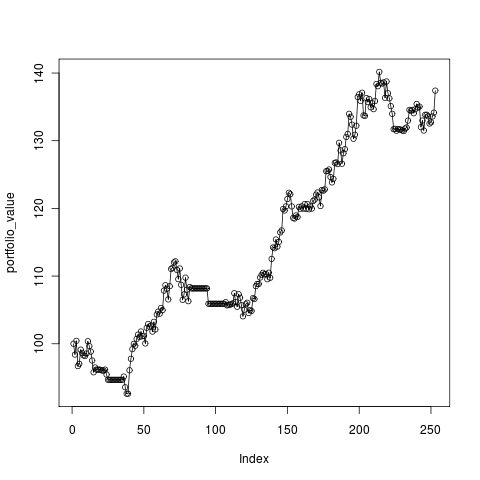
\includegraphics[scale=.4]{rplot0.png}
  \end{center}
  \caption{Chart showing value of our portfolio in time}
  \label{fig:trend-short}
\end{figure}

There are easily visible periods of time (figure~\ref{fig:trend-short}) when the portfolio value is not changing. 
It is a time when our portfolio does not contain any assets (but we still have money). 
After a while, conditions change and trend following algorithm decides to buy some assets.


\subsubsection{Intermediate-term trend results}

In this particular test (with values: $N = 20$, $M = 40$), trend following algorithm has been adjusted to focus on intermediate-term trends.
 
\begin{figure}[H]
  \begin{center}
    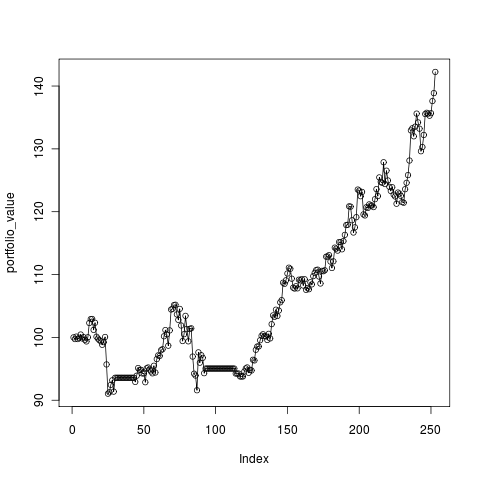
\includegraphics[scale=.4]{rplot.png}
  \end{center}
  \caption{Chart showing value of our portfolio in time}
  \label{fig:trend-int}
\end{figure}

Results are presented in figure~\ref{fig:trend-int}, as can be seen they are slightly better compared with short-term trends approach.  

\subsubsection{Conclusions}

It turned out that focusing on short-term or intermediate-term trends leads to almost the same results.
Intermediate-term trend approach offers slightly better return from the investment.
In both cases we encountered periods of time when portfolio contained no assets because situation on the market was not good enough to invest in any of the available stocks.


%---------------------------------------------------------------------------

\subsection{Genetic Algorithm}

Results are presented in figure ~\ref{fig:gen-algo}.

\begin{figure}[ht]
  \begin{center}
    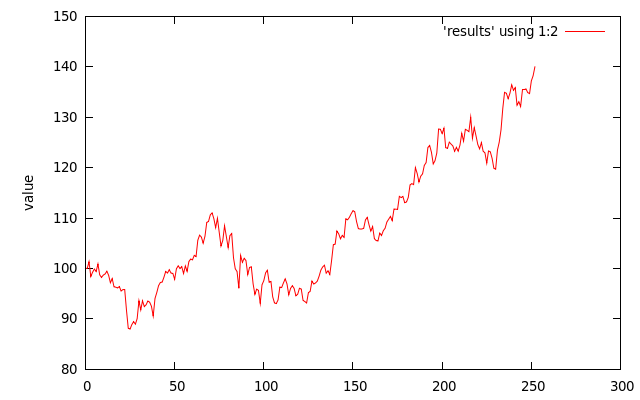
\includegraphics[scale=.5]{simple-genetic-algo.png}
  \end{center}
  \caption{Chart showing value of our portfolio in time}
  \label{fig:gen-algo}
\end{figure}

\subsection{Co-evolutionary algorithm}
\label{sec:co-evol-2}

Results presented in figure~\ref{fig:co_eval_return} clearly show that the return of our investment is much higher than any other algorithm could achieve.  
Analysing figure~\ref{fig:co_eval_risk} explains why the results are so good - the risk associated with our portfolio is substantially higher compared to other methods.
In this case algorithm was tuned to treat non-dominated solutions from return oriented subpopulation - this explains why the results provide so much return and risk. 

\begin{figure}[ht]
  \begin{center}
    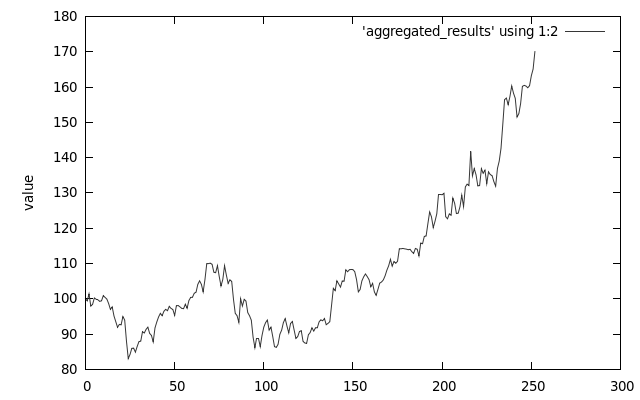
\includegraphics[scale=.5]{co-evol-value-oriented.png}
  \end{center}
  \caption{Chart showing value of our portfolio in time}
  \label{fig:co_eval_return}
\end{figure}

\subsubsection{Pareto front}

Because co-evolutionary algorithm operates in terms of risk and return we can check if the non dominated solutions (in Pareto sense) are used to construct our portfolio.
Figure~\ref{fig:pareto_co_evol} shows the results of computation (results from a period of 6 days are presented for the sake of clarity). 
Portfolio is built according to the solutions that are connected with red line.
All of them are non dominated and all have the maximum return possible from all available feasible solutions at any particular day.

Solutions from two different computing nodes are shown.
It turns out that results from the second node are much better than from the first.
In fact all of the selected solutions come from the second one.

\begin{figure}[ht]
  \begin{center}
    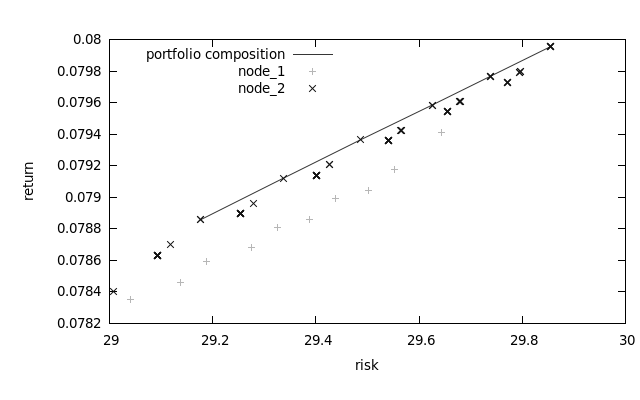
\includegraphics[scale=.5]{pareto_co_evol.png}
  \end{center}
  \caption{Chart showing the relation between return and risk of the particular solution}
  \label{fig:pareto_co_evol}
\end{figure}


\begin{figure}[ht]
  \begin{center}
    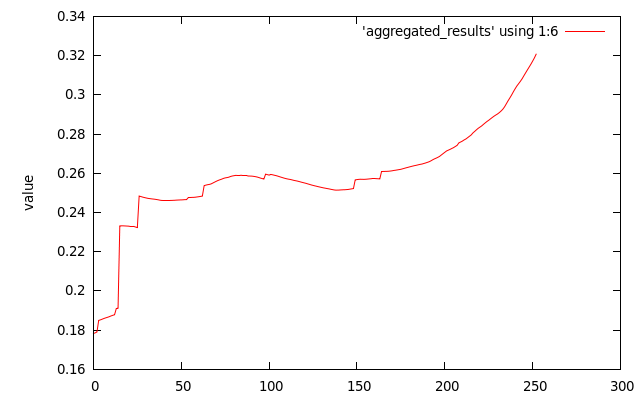
\includegraphics[scale=.5]{co-evol-risk-value-oriented.png}
  \end{center}
  \caption{Chart showing value of risk in time}
  \label{fig:co_eval_risk}
\end{figure}

\subsection{CoEMAS}

Figure~\ref{fig:agent_return} presents portfolio value in time while  figure~\ref{fig:agent_risk} presents the risk associated with our investments.

\begin{figure}[ht]
  \begin{center}
    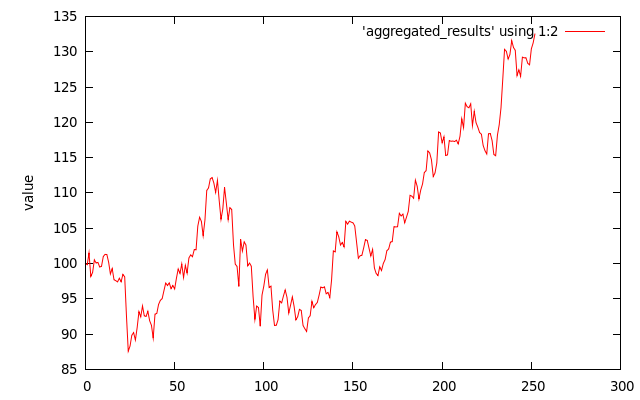
\includegraphics[scale=.5]{agent-return.png}
  \end{center}
  \caption{Chart showing value of our portfolio in time (CoEMAS)}
  \label{fig:agent_return}
\end{figure}

\subsubsection{Pareto front}

CoEMAS like co-evolutionary algorithm gives us the opportunity to check if the non dominated solutions (in Pareto sense) are used to construct our portfolio.
Figure~\ref{fig:pareto_coemas} shows the results of computation (because of the fact that populations are quite numerous,
 results from a period of 3 days are presented for the sake of clarity). 
Solutions chosen to be a blueprint for our portfolio are shown as big black dots.
We can easily spot that they are non dominated (in Pareto sense). 


\begin{figure}[ht]
  \begin{center}
    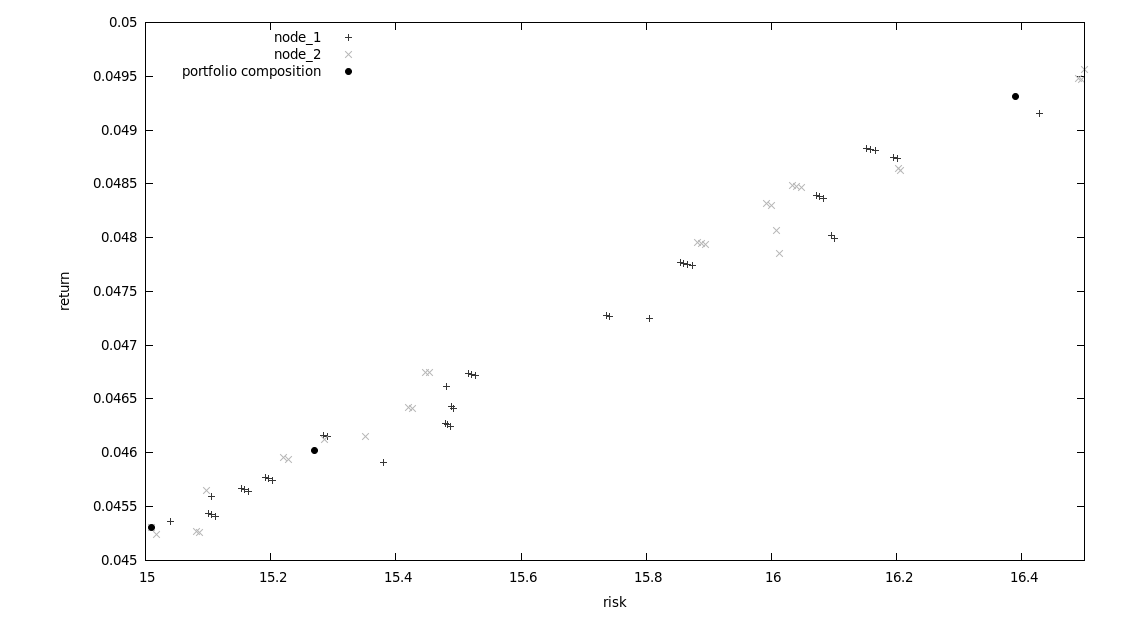
\includegraphics[scale=.4]{pareto_coemas.png}
  \end{center}
  \caption{Chart showing the relation between return and risk of the particular solution}
  \label{fig:pareto_coemas}
\end{figure}

\begin{figure}[ht]
  \begin{center}
    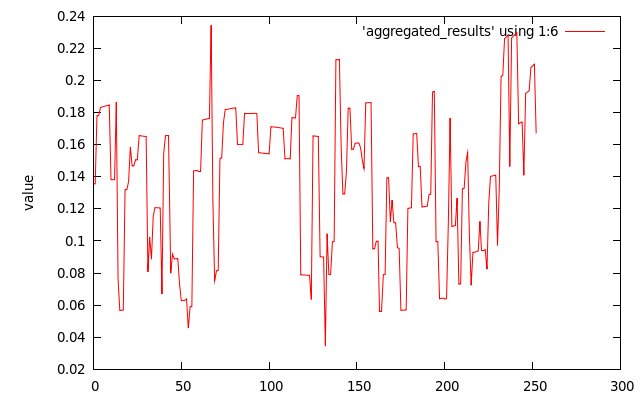
\includegraphics[scale=.5]{agent-risk.png}
  \end{center}
  \caption{Chart showing value of risk in time (CoEMAS)}
  \label{fig:agent_risk}
\end{figure}

\subsection{Conclusions}

First set of tests showed that all algorithms give reasonable results.
It is very hard to pinpoint one approach that is much better than others.
Co-evolutionary system (\ref{sec:co-evol-sys}) outperformed other algorithms in terms of return.
Such good results can be explained by the fact that trading strategy proposed by this algorithm is much riskier than using CoEMAS.
  
On the other hand, CoEMAS offers substantially lower return but is much more safer.
As figure~\ref{fig:agent_risk} shows, the risky moves are mixed with safe ones resulting in much more balanced strategy.

Trend following as well as genetic algorithm can not give us any information about the risk we are taking by investing according to results they provide.
On the other hand, we can specify rules (in the trend following approach) that should reflect our attitude to risk taking (\ref{sec:trend_following_fundamentals}).
With genetic algorithm (GA) we have no such option - as described in \ref{sec:gen_fitness_fun}, our ability to customize GA is limited.
Obviously we could test different values of coefficients responsible for simulating evolution process but it turns out that the fitness function that does not take risk into
account is the most serious limitation.


\section{Second Set of Tests}

The main goal of this set of tests is to chech the impact of increasing the number of computing nodes to the quality of solutions we obtain from implemented algorithms.

Besides the number of computing nodes (now 8 computing nodes will be running at once), the same historical data and configuration has been
 used (as in \ref{sec:first_set_of_tests}) to produce results.



\subsection{Co-evolutionary algorithm}

Figure~\ref{fig:co_evol_8_risk} presents risk associated with our portfolio.


Comparing with results presented in \ref{sec:co-evol-2} we can easily spot that additional computing nodes allowed us to find a solution that is much more risk free.
Apart from that higher number of nodes offer similar performance in terms of return (figure~\ref{co_evol_8_return}).

\begin{figure}[ht]
  \begin{center}
    \includegraphics[scale=.5]{co-evol-8.png}
  \end{center}
  \caption{Chart showing value of risk in time}
  \label{fig:co_evol_8_risk}
\end{figure}

\begin{figure}[ht]
  \begin{center}
    \includegraphics[scale=.5]{co_evol_8_return.png}
  \end{center}
  \caption{Chart showing portfolio value in time}
  \label{fig:co_evol_8_return}
\end{figure}

\subsection{CoEMAS}

\begin{figure}[ht]
  \begin{center}
    \includegraphics[scale=.5]{agent_8_risk.png}
  \end{center}
  \caption{Chart showing portfolio value in time}
  \label{fig:agent_8_risk}
\end{figure}

In case of CoEMAS adding more computing nodes seems to have little effect.
Risk associated with our portfolio is almost the same as before (figure~\ref{fig:agent_8_risk}).
There is no significant improvement in terms of return (as shown in figure~\ref{fig:agent_8_return}). 


\begin{figure}[ht]
  \begin{center}
    \includegraphics[scale=.5]{agent_return_8.png}
  \end{center}
  \caption{Chart showing portfolio value in time}
  \label{fig:agent_8_return}
\end{figure}

\subsection{Conclusions}

Adding additional computing nodes tends to improve the performance of co-evolutionary algorithm, whereas there is almost no impact on CoEMAS.
It can be explained by the fact that each CoEMAS node has a significantly large and diverse population that is not prone to fall in local minima.
Co-evolutionary algorithm benefits a lot from a larger number of computing nodes.  

\section{Third Set of Tests}

\subsection{Trend Following}

\subsubsection{Short-term trend results}
\subsubsection{Intermediate-term trend results}
\subsubsection{Conclusions}

\subsection{Genetic Algorithm}

\subsection{Co-evolutionary algorithm}

\subsection{CoEMAS}


\subsection{Conclusions}